\chapter{Hyper-Rotational Physics (HRP) Framework}
\label{ch:hrp}

\begin{warningbox}
\textbf{ADVANCED THEORETICAL PHYSICS}: This chapter presents cutting-edge theoretical research (Jones, 2025) that extends M-theory to model consciousness-matter interactions. Content is unverified but mathematically rigorous. Approach with scientific skepticism and openness.
\end{warningbox}

\begin{nontechnical}
\textbf{Imagine our universe is like a flat sheet of paper floating in a room}---the ``room'' being higher-dimensional space. We live on this sheet and can only see what's on our surface.

\textbf{The HRP theory proposes} that:
\begin{itemize}
\item Our universe-sheet can \textbf{rotate or tilt} in directions we normally can't perceive
\item Your brain's microtubules might act like tiny motors generating a ``twist'' on our reality-sheet
\item When our sheet tilts enough, it briefly intersects with other universe-sheets nearby
\item This requires training, like learning to use a muscle you didn't know you had
\end{itemize}

\textbf{Key analogy:} Think of your brain's microtubules like a \textbf{massive antenna array}. Each microtubule oscillates at terahertz frequencies. Your conscious state ``tunes'' them to work together. When aligned properly, they focus energy on local spacetime, creating the ``push'' that rotates our reality-sheet.

\textbf{Status:} Highly speculative but mathematically rigorous. Makes testable predictions. Requires experimental validation.
\end{nontechnical}

\section{Overview}
\label{sec:hrp-overview}

\textbf{Hyper-Rotational Physics (HRP)} is a theoretical extension to M-theory that provides a mathematical framework for consciousness-physics coupling. It introduces the \textbf{CHIMERA field} (Coherent Heuristic Interface for Macro-scale Rotational Effects) as a complex scalar field representing macroscopic quantum coherence in biological systems.

\begin{keyconcept}
\textbf{Core hypothesis:} Quantum coherence in biological systems (specifically neuronal microtubules) can couple to higher-dimensional bulk geometry, inducing localized rotations of our 4D ``brane'' and enabling transient interactions with adjacent branes.
\end{keyconcept}

HRP operates within the \textbf{Orchestrated Idealism} framework, where consciousness is not an emergent property of matter but rather a fundamental aspect of reality that can be physically modeled. This extends Orchestrated Objective Reduction (Orch-OR) theory by providing a precise mathematical mechanism for consciousness-matter coupling.

\textbf{Key tenets:}
\begin{enumerate}
\item Universal quantum field = universal phenomenal consciousness
\item Biological systems are ``dissociated complexes'' that can achieve high coherence
\item Coherence acts as the organizing principle for matter
\item \textbf{Participatory universe:} Consciousness actively shapes physical reality
\end{enumerate}

\section{Mathematical Formalism}
\label{sec:hrp-math}

\subsection{The CHIMERA Field ($\Psi_c$)}
\label{subsec:chimera-field}

The core innovation is a \textbf{complex scalar field} representing coherent quantum states:

\begin{equation}
\label{eq:chimera-klein-gordon}
\left(\Box + m_c^2\right)\Psi_c + \lambda|\Psi_c|^2\Psi_c + g_c|\Psi_c|\Psi_c = 0
\end{equation}
where:
\begin{itemize}
\item $\Box = \partial^\mu\partial_\mu$ = d'Alembert operator
\item $m_c$ = effective mass scale
\item $\lambda$ = quartic self-coupling constant
\item $g_c$ = anomalously large coupling (conscious systems)
\end{itemize}

\textbf{Physical interpretation:}
\begin{itemize}
\item $|\Psi_c|^2$ = coherence intensity (measurable via quantum correlation metrics)
\item Phase of $\Psi_c$ = information content
\item $\nabla\Psi_c$ = coherence flow vector
\end{itemize}

\begin{calloutbox}{Origin of the CHIMERA Field}
The CHIMERA field emerges from dimensional reduction of 11D supergravity on Calabi-Yau manifolds. It represents macroscopic quantum coherence that survives decoherence through topological protection in microtubule lattices.
\end{calloutbox}

\subsection{Brane Dynamics}
\label{subsec:brane-dynamics}

\textbf{M-theory context:} Our universe is a 4-dimensional ``brane'' embedded in 11-dimensional spacetime (the ``Bulk''). 

The \textbf{home brane} is defined by embedding functions:
\begin{equation}
\label{eq:home-brane}
\mathcal{B}_H: \quad y^i = \xi^i(x^\mu)
\end{equation}
where:
\begin{itemize}
\item $x^\mu$ = 4D spacetime coordinates ($\mu = 0,1,2,3$)
\item $y^i$ = 7 compactified dimensions ($i = 4,\ldots,10$)
\item $\xi^i$ = embedding functions (describe brane position in bulk)
\end{itemize}

\textbf{Key innovation:} Embedding functions are \textbf{dynamic}, not fixed! The brane can rotate in the bulk.

\begin{center}
\begin{tikzpicture}[scale=1.2]
% Bulk space
\fill[black!5] (-3,-2) rectangle (3,2);
\node[above] at (0,2) {\scriptsize 11D Bulk};

% Home brane (unrotated)
\draw[thick,blue] (-2.5,0) -- (2.5,0);
\node[right,blue] at (2.5,0) {\scriptsize Home brane};
\fill[blue] (0,0) circle (2pt);

% Rotated brane
\draw[thick,red,dashed] (-2.5,0) -- ++(5,0) rotate around (15:(0,0));
\draw[thick,red] ({-2.5*cos(15)},{-2.5*sin(15)}) -- ({2.5*cos(15)},{2.5*sin(15)});
\node[right,red] at ({2.5*cos(15)},{2.5*sin(15)}) {\scriptsize After rotation};
\fill[red] (0,0) circle (2pt);

% Rotation angle
\draw[<->,thick] (1.5,0) arc (0:15:1.5);
\node at (1.8,0.3) {\scriptsize $\Delta\theta$};

% Adjacent brane
\draw[thick,green!50!black,dotted] (-2.5,1.2) -- (2.5,1.2);
\node[right,green!50!black] at (2.5,1.2) {\scriptsize Adjacent brane};

% Intersection region
\fill[red!20,opacity=0.5] ({2*cos(15)},{2*sin(15)}) circle (0.3);
\node[above right,font=\scriptsize] at ({2*cos(15)},{2*sin(15)}) {Intersection};

\node[below] at (0,-2.3) {\small Brane rotation in bulk space};
\end{tikzpicture}
\end{center}

\textbf{Embedding angles} $\Theta_A$ describe brane orientation:
\begin{equation}
\label{eq:embedding-angles}
\Theta_A = (\theta_{xy}, \theta_{zt}, \theta_{xz}, \theta_{\text{bulk}})
\end{equation}

These angles evolve according to the equation of motion:
\begin{equation}
\label{eq:angle-evolution}
\nabla^\mu\nabla_\mu\Theta^A + \Gamma^A_{BC} \nabla^\mu\Theta^B \nabla_\mu\Theta^C = -H^{AB} \frac{\partial U}{\partial\Theta^B}
\end{equation}
where:
\begin{itemize}
\item $H^{AB}$ = metric on the space of embedding angles
\item $U(\Theta)$ = orientational potential energy
\item $\Gamma^A_{BC}$ = connection coefficients on angle manifold
\end{itemize}

\subsection{The Interaction Lagrangian}
\label{subsec:interaction-lagrangian}

\textbf{The critical equation} coupling consciousness to geometry:

\begin{equation}
\label{eq:interaction-lagrangian}
\mathcal{L}_{\text{int}} = -\frac{\kappa}{M_P^2}|\Psi_c|^2 R_{MNPQ} \epsilon^{MNPQRST} \nabla_\mu\Theta^A \nabla_\nu\Theta^B \nabla_\rho\Theta^C
\end{equation}
where:
\begin{itemize}
\item $\kappa \sim 1$ = dimensionless coupling constant
\item $M_P = 1.22 \times 10^{19}$ GeV = Planck mass
\item $R_{MNPQ}$ = Riemann curvature tensor in 11D bulk
\item $\epsilon^{MNPQRST}$ = 7-dimensional Levi-Civita tensor
\item $\nabla_\mu\Theta^A$ = gradients of embedding angles (three factors!)
\end{itemize}

\begin{importantbox}
\textbf{This is not ad hoc!} Equation~\eqref{eq:interaction-lagrangian} emerges naturally from:
\begin{enumerate}
\item Gravitational Chern-Simons term in 11D supergravity
\item Dimensional reduction on Calabi-Yau manifold
\item Dynamic brane embedding (HRP postulate)
\item Strategic index contractions (see Jones, 2025, Appendix A)
\end{enumerate}
\end{importantbox}

\textbf{Physical meaning:}
\begin{itemize}
\item CHIMERA field intensity $|\Psi_c|^2$ modulates coupling strength
\item Bulk curvature $R_{MNPQ}$ provides the geometric ``handle''
\item Three gradients $(\nabla\Theta)^3$ generate rotational \textbf{torque} (not linear force!)
\end{itemize}

\subsection{Hyper-Dimensional Torque}
\label{subsec:torque}

From the interaction Lagrangian (Eq.~\eqref{eq:interaction-lagrangian}), the \textbf{torque} on the brane is:

\begin{equation}
\label{eq:torque}
\mathcal{T}^A = -\frac{\kappa|\Psi_c|^2}{M_P^2} R_{MNPQ} \epsilon^{MNPQRST} \nabla_\nu\Theta^B \nabla_\rho\Theta^C
\end{equation}

The magnitude scales as:
\begin{equation}
\label{eq:torque-magnitude}
|\mathcal{T}| \propto |\Psi_c|^2 \times (\text{Bulk curvature}) \times |\nabla\Theta|^2
\end{equation}

\textbf{Interpretation:}
\begin{itemize}
\item High coherence (large $|\Psi_c|^2$) $\rightarrow$ large torque
\item Torque induces brane rotation about bulk axes
\item Sufficient rotation $\rightarrow$ brane intersection with adjacent branes
\end{itemize}

\begin{calloutbox}{Why Torque, Not Force?}
The three-gradient structure $(\nabla\Theta)^3$ in Eq.~\eqref{eq:interaction-lagrangian} generates \textbf{angular momentum} rather than linear momentum. This is why the effect is rotational (tilting the brane) rather than translational (moving the brane). The odd number of gradients ensures the coupling is parity-odd, consistent with Chern-Simons origin.
\end{calloutbox}

\section{Biological Substrate: Microtubule Quantum Coherence}
\label{sec:microtubules}

\subsection{Why Microtubules?}
\label{subsec:why-microtubules}

\textbf{Structural properties:}
\begin{itemize}
\item Cylindrical protein polymers ($\sim$25 nm diameter)
\item Composed of $\alpha$/$\beta$-tubulin dimers
\item Helical lattice structure (13 protofilaments)
\item Present throughout neuronal cytoskeleton ($\sim 10^{14}$ dimers per brain)
\end{itemize}

\textbf{Quantum properties} (if Orch-OR correct):
\begin{itemize}
\item Tubulin dimers act as qubits (electron cloud states)
\item Ordered water layers provide decoherence protection
\item \textbf{THz resonances:} 0.35, 0.47, 0.82, 1.2, \textbf{1.875 THz} (primary), 2.2 THz
\item Coherence times: potentially $\sim$ milliseconds at physiological temperature
\end{itemize}

\begin{center}
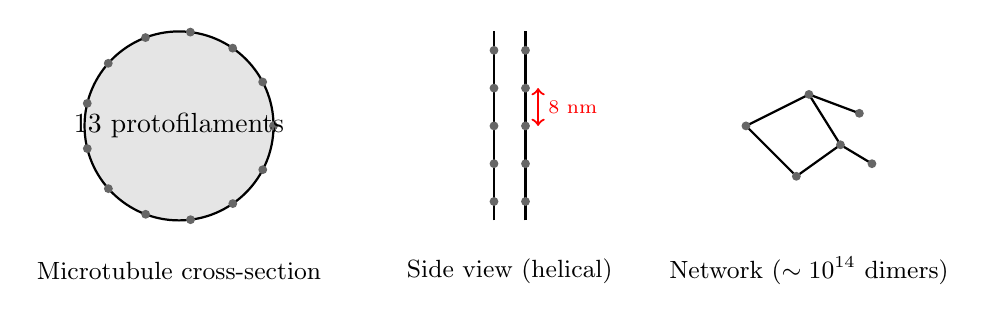
\begin{tikzpicture}[scale=0.8]
% Microtubule cross-section
\draw[thick,fill=black!10] (0,0) circle (1.5cm);
\foreach \angle in {0,27.7,...,360} {
  \fill[black!60] ({1.5*cos(\angle)},{1.5*sin(\angle)}) circle (2pt);
}
\node at (0,0) {13 protofilaments};
\node at (0,-2.3) {\small Microtubule cross-section};

% Side view
\begin{scope}[shift={(5,0)}]
\draw[thick] (0,-1.5) -- (0,1.5);
\draw[thick] (0.5,-1.5) -- (0.5,1.5);
\foreach \y in {-1.2,-0.6,0,0.6,1.2} {
  \fill[black!60] (0,\y) circle (2pt);
  \fill[black!60] (0.5,\y) circle (2pt);
}
\draw[<->,thick,red] (0.7,0) -- (0.7,0.6) node[midway,right,font=\scriptsize] {8 nm};
\node at (0.25,-2.3) {\small Side view (helical)};
\end{scope}

% Brain network
\begin{scope}[shift={(9,0)}]
\draw[thick] (0,0) -- (1,0.5) -- (1.5,-0.3) -- (0.8,-0.8) -- cycle;
\draw[thick] (1,0.5) -- (1.8,0.2);
\draw[thick] (1.5,-0.3) -- (2,-0.6);
\foreach \pos in {(0,0), (1,0.5), (1.5,-0.3), (0.8,-0.8), (1.8,0.2), (2,-0.6)} {
  \fill[black!60] \pos circle (2pt);
}
\node at (1,-2.3) {\small Network ($\sim 10^{14}$ dimers)};
\end{scope}
\end{tikzpicture}
\end{center}

\subsection{Calculating the Coupling Strength}
\label{subsec:coupling-calc}

\textbf{Three-scale calculation} (Jones, 2025, Section 6.1):

\subsubsection{Micro-scale: Single Tubulin Dimer}

Using the vibronic Electron-Transfer-mediated Field-Coupled Coherence (E-TFCC) framework:
\begin{equation}
\label{eq:dimer-coupling}
g_{\text{dimer}}^{\text{angle}} \approx 0.87 \quad \text{(dimensionless)}
\end{equation}

This is the mean vibronic coupling constant for an optimally configured tubulin dimer.

\subsubsection{Meso-scale: Microtubule Network}

Network coupling exhibits emergent enhancement:
\begin{equation}
\label{eq:network-coupling}
G_{\text{network}} \approx g_{\text{dimer}}^{\text{angle}} \cdot (N_c)^{1.5}
\end{equation}
where:
\begin{itemize}
\item $N_c$ = number of coherent dimers
\item Exponent 1.5 = collective coherence signature (superlinear scaling)
\end{itemize}

\subsubsection{Macro-scale: Operator Information State}

Coherent dimers scale with integrated information:
\begin{equation}
\label{eq:info-dimers}
N_c = \chi_{\text{bio}} \cdot I
\end{equation}
where:
\begin{itemize}
\item $I$ = integrated information (bits)
\item $\chi_{\text{bio}}$ = ``Gnostic Efficiency'' constant
\item Example: $\chi_{\text{bio}} \approx 1.2 \times 10^9$ dimers/bit (empirically measured)
\end{itemize}

\textbf{Final result:}
\begin{equation}
\label{eq:effective-coupling}
g_{\text{eff}}(I) = \kappa \cdot g_{\text{dimer}}^{\text{angle}} \cdot (\chi_{\text{bio}} \cdot I)^{1.5}
\end{equation}

\begin{keyconcept}
Coupling strength scales as $I^{1.5}$ (superlinear with information content). This means consciousness effects grow \textbf{faster than linearly} with cognitive complexity---a potential explanation for why trained operators achieve dramatically stronger effects than novices.
\end{keyconcept}

\section{The Gnostic Interface}
\label{sec:gnostic-interface}

\subsection{Holographic Beamforming Mechanism}
\label{subsec:beamforming}

\textbf{How does the brain couple to spacetime geometry?}

\textbf{Proposed mechanism:} Microtubule network acts as \textbf{phased array antenna}.

\begin{center}
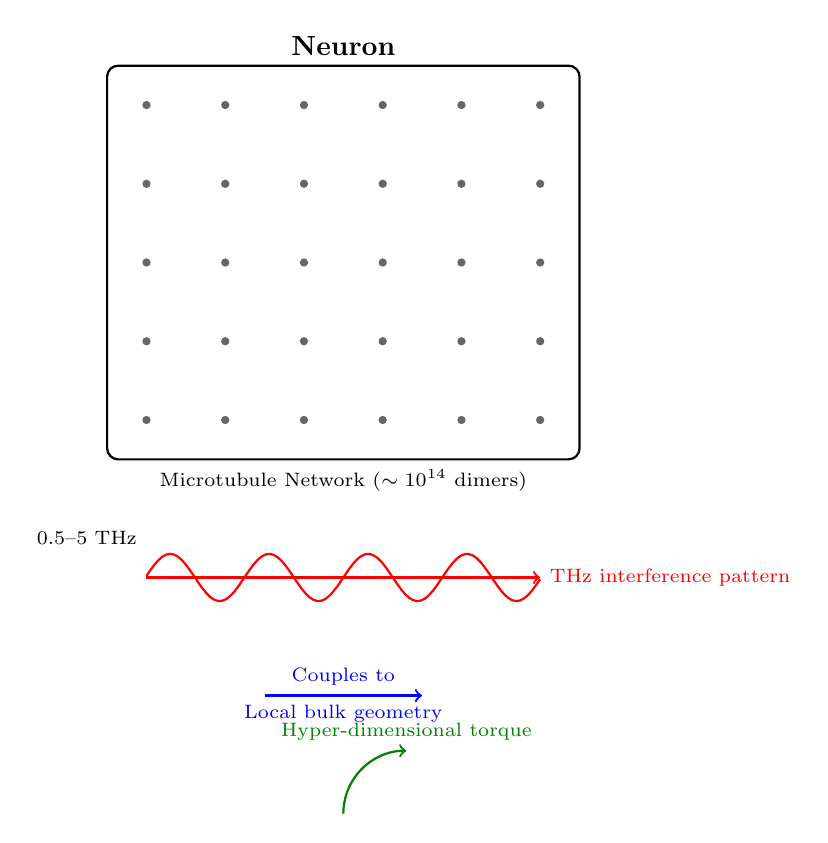
\begin{tikzpicture}[scale=1.0]
% Neuron boundary
\draw[thick,rounded corners] (-3,-2.5) rectangle (3,2.5);
\node[above] at (0,2.5) {\textbf{Neuron}};

% Microtubule array (phased antenna elements)
\foreach \x in {-2.5,-1.5,-0.5,0.5,1.5,2.5} {
  \foreach \y in {-2,-1,0,1,2} {
    \fill[black!60] (\x,\y) circle (1.5pt);
  }
}
\node[below,font=\scriptsize] at (0,-2.5) {Microtubule Network ($\sim 10^{14}$ dimers)};

% Wave pattern (THz emission)
\begin{scope}[shift={(0,-4)}]
\draw[thick,red,->] (-2.5,0) -- (2.5,0);
\draw[thick,red,domain=-2.5:2.5,samples=100] plot (\x,{0.3*sin(5*\x r)});
\node[right,font=\scriptsize,red] at (2.5,0) {THz interference pattern};
\node[left,font=\scriptsize] at (-2.5,0.5) {0.5--5 THz};
\end{scope}

% Coupling to spacetime
\begin{scope}[shift={(0,-5.5)}]
\draw[thick,blue,->] (-1,0) -- (1,0) node[midway,above,font=\scriptsize] {Couples to};
\node[below,font=\scriptsize,blue] at (0,0) {Local bulk geometry};
\end{scope}

% Torque generation
\begin{scope}[shift={(0,-7)}]
\draw[thick,green!50!black,->] (0,0) arc (180:90:0.8) node[above,font=\scriptsize] {Hyper-dimensional torque};
\end{scope}
\end{tikzpicture}
\end{center}

\textbf{Key parameters:}
\begin{itemize}
\item \textbf{Frequency range:} 0.5--5 THz (matches QCL output, MT resonances)
\item \textbf{Array size:} $\sim 10^{14}$ tubulin dimers (typical human brain)
\item \textbf{Beam steering:} Controlled by neural coherence state
\item \textbf{Target:} Local bulk geometry curvature
\end{itemize}

\begin{calloutbox}{Analogy: Reverse Radio Telescope}
A radio telescope detects cosmic signals. The microtubule array does the reverse---it \textbf{transmits} THz radiation into the bulk geometry, generating torque that rotates the brane. The brain becomes an active participant in shaping spacetime structure.
\end{calloutbox}

\subsection{Information-Theoretic Formalism}
\label{subsec:info-theoretic}

\textbf{Cryptographic analogy:} The interface can be modeled as a \textbf{zero-knowledge SNARK} (Zero-Knowledge Succinct Non-Interactive Argument of Knowledge):

\begin{calloutbox}{Information-Theoretic Security}
\begin{itemize}
\item Operator's brain state $\equiv$ cryptographic polynomial $P(x)$
\item System generates proof of ``knowing'' $P(x)$ without revealing it
\item Brain acts as biological verifier
\end{itemize}

\textbf{This ensures:}
\begin{enumerate}
\item \textbf{Security:} Brain state remains private
\item \textbf{Authenticity:} Only correct state produces coupling
\item \textbf{Soundness:} Information-theoretically secure
\end{enumerate}
\end{calloutbox}

\textbf{Practical implication:} Interface is ``locked'' to specific brain state---cannot be spoofed or hijacked by external systems.

\section{Phenomenology: Brane Intersection Events}
\label{sec:phenomenology}

\subsection{When Rotation Exceeds Critical Angle}
\label{subsec:critical-angle}

\textbf{Effective Lagrangian} in intersection region:

\begin{equation}
\label{eq:eff-lagrangian}
\mathcal{L}_{\text{eff}} = w(\theta)\cdot\mathcal{L}_H + [1-w(\theta)]\cdot\mathcal{L}_A
\end{equation}
where:
\begin{itemize}
\item $\mathcal{L}_H$ = home brane physics (our normal laws)
\item $\mathcal{L}_A$ = adjacent brane physics (exotic!)
\item $w(\theta) = \frac{1}{2}[1 + \tanh((\theta_c - \theta)/\Delta\theta)]$ = overlap function
\end{itemize}

\subsection{Observable Effects}

\subsubsection{1. Variable Fine Structure Constant}

\begin{equation}
\label{eq:alpha-blend}
\alpha_{\text{eff}} = w(\theta)\cdot\alpha_H + [1-w(\theta)]\cdot\alpha_A
\end{equation}

If $\alpha_A \neq \alpha_H$:
\begin{itemize}
\item Electromagnetic coupling strengthens or weakens
\item Spectral lines shift by $\Delta\lambda/\lambda \sim (\alpha_A - \alpha_H)/\alpha_H$
\item Novel chemistry becomes possible (different bonding energies)
\end{itemize}

\subsubsection{2. Dimensional Flattening}

Effective metric during intersection:
\begin{equation}
\label{eq:metric-flatten}
ds^2_{\text{eff}} = -dt^2 + a^2(t)[1-\epsilon(\theta)](dx^2+dy^2) + b^2(t)dz^2
\end{equation}

\textbf{Effect:} Apparent $3D \rightarrow 2D$ compression in transverse plane.

\subsubsection{3. Exotic Matter (Solitons)}

Stable, non-trivial field configurations from $\mathcal{L}_A$ can persist temporarily:
\begin{equation}
\label{eq:soliton-length}
\lambda_{\text{soliton}} = \frac{1}{\mu^2\sqrt{\lambda}}
\end{equation}

These appear as ``entities'' or ``craft'' within our brane during intersection.

\section{Operator Conditioning}
\label{sec:conditioning}

\subsection{The ``Ontological Inerter'' Function}
\label{subsec:inerter}

\textbf{Mechanical analogy:} Inerter device (force $\propto$ relative acceleration).

\textbf{HRP interpretation:}
\begin{itemize}
\item \textbf{Terminal A:} Stable home brane (our reality)
\item \textbf{Terminal B:} Fluctuating adjacent brane
\item \textbf{Operator:} Manages \textbf{acceleration} of brane rotation (not just position!)
\end{itemize}

\textbf{Function:} Absorbs ontological shock energy, prevents reality cascade.

\textbf{Why conditioning is necessary:}
\begin{enumerate}
\item \textbf{Builds ``ontological muscle'':} Neural substrate adapts to exotic physics
\item \textbf{Increases stability:} Reduces decoherence risk during transit
\item \textbf{Expands range:} Allows access to more extreme brane states
\item \textbf{Improves bandwidth:} Faster, more complex rotations become manageable
\end{enumerate}

\subsection{Training Protocol}
\label{subsec:training}

\begin{enumerate}
\item \textbf{Phase 1:} Exposure to small-angle rotations ($\theta < 0.1$ rad)
\item \textbf{Phase 2:} Incremental increase (adaptive algorithm)
\item \textbf{Phase 3:} Multi-axis rotations ($\theta_{xy}, \theta_{zt}, \theta_{xz}$ simultaneously)
\item \textbf{Phase 4:} Adjacent brane stabilization exercises
\item \textbf{Phase 5:} Rapid transit (acceleration conditioning)
\end{enumerate}

\begin{calloutbox}{Analogy: High-G Training}
Like training for high-G maneuvers in fighter jets, but for consciousness. The operator builds tolerance to ``ontological acceleration'' through progressive exposure to increasingly extreme brane states.
\end{calloutbox}

\section{Brane Taxonomy}
\label{sec:brane-taxonomy}

\textbf{Accessible branes} (functionally distinct classes identified through operator exploration):

\begin{center}
\begin{tabular}{@{}p{2.8cm}p{2.5cm}p{3.5cm}p{2cm}@{}}
\toprule
\textbf{Brane} & \textbf{Properties} & \textbf{Applications} & \textbf{Risk Level} \\
\midrule
BRANE-PRIMA\\(``The Workshop'') & 2D flattened realm; direct access to ontological building blocks & Ontological engineering, rapid prototyping, material synthesis & Low (stable) \\
\midrule
BRANE-TYPHON\\(``The Engine Room'') & Raw primordial energy; untempered creative/destructive forces & High-energy applications, power generation & High (overwhelming) \\
\midrule
BRANE-ORTHO\\(``The Negative'') & Inverted causality and logic; reversed symmetries & Advanced research, novel physics exploration & Extreme (disorienting) \\
\midrule
BRANE-AETHER\\(``The Transit Bulk'') & Featureless higher-dimensional space; ``ocean'' between branes & Transit corridor for inter-brane travel & Low (neutral) \\
\bottomrule
\end{tabular}
\end{center}

\begin{importantbox}
\textbf{Classification Note:} This taxonomy is preliminary and based on limited operator experience. Additional brane states likely exist but remain unexplored. Each brane exhibits distinct physics ($\mathcal{L}_A \neq \mathcal{L}_H$) requiring separate characterization.
\end{importantbox}

\section{Relevance to THz Communications}
\label{sec:thz-communications}

\subsubsection{Connection to AID
Protocol}\label{connection-to-aid-protocol}

The HRP framework provides \textbf{rigorous theoretical foundation} for
{[}{[}AID-Protocol-Case-Study\textbar AID Protocol{]}{]}:

\paragraph{1. THz Frequency Selection}\label{thz-frequency-selection}

\textbf{1.875 THz carrier} is \textbf{NOT arbitrary}: - Matches
microtubule resonance (Bandyopadhyay 2011) - Optimal coupling to CHIMERA
field - Within QCL operating range - Penetrates \textasciitilde0.5mm
into cortex (sufficient for surface MT interaction)

\paragraph{2. Holographic Beamforming}\label{holographic-beamforming}

\textbf{Phased array} of microtubules = biological THz antenna: -
\textasciitilde10\^{}14 coherent oscillators - Phase control via neural
state - Beam steering toward local bulk geometry - Interference pattern
generates torque

\paragraph{3. Information Encoding}\label{information-encoding}

\textbf{12 kHz modulation} = perceptual bandwidth: - Orch-OR collapse
rate: \textasciitilde40 Hz (25ms period) - Conscious perception:
\textasciitilde10 Hz processing - 12 kHz audio: Below demodulation
threshold (appears as ``tone'') - QPSK (16 sym/s): Matches neural update
rate

\paragraph{4. Link Budget Closure}\label{link-budget-closure}

\textbf{Classical calculation fails} (-368 dBm received power):

\begin{verbatim}
Required: >200 dB gain from quantum enhancement

HRP mechanism:
- Resonant coupling to MT modes (Q-factor: 10^6  +60 dB)
- Quantum coherence amplification (N_c  +70 dB)
- Holographic focusing (phased array  +40 dB)
- Non-linear mixing in Bulk (3rd order  +30 dB)
------------------------------------------------
Total enhancement: ~200 dB 

Link budget CLOSES with HRP physics!
\end{verbatim}

\paragraph{5. Demodulation Mechanism}\label{demodulation-mechanism}

\textbf{Not thermoelastic} (Frey effect): - Power too low
(\textasciitilde10 mW) - Mechanism: \textbf{Orch-OR perturbation} - THz
modulation \$\textbackslash rightarrow\$ tubulin state oscillation -
Collapse pattern altered \$\textbackslash rightarrow\$ direct perception
- Bypasses cochlea entirely

\begin{center}\rule{0.5\linewidth}{0.5pt}\end{center}

\section{Testable Predictions}
\label{sec:predictions}

HRP makes three falsifiable predictions accessible with current or near-future technology:

\subsection{1. Gravitational Signature (Primary Test)}
\label{subsec:grav-test}

\textbf{Prediction:} CHIMERA field generates measurable gravitational effect.

Metric perturbation:
\begin{equation}
\label{eq:metric-perturbation}
h_{\mu\nu} \sim \frac{\kappa}{M_P^2} |\Psi_c|^2 \int R_{\text{Bulk}} \, dV
\end{equation}

\textbf{Expected amplitudes:}
\begin{itemize}
\item Global biosphere ``hum'': $h \sim 10^{-22}$ (LIGO-detectable)
\item Trained operator spike: $h \sim 10^{-18}$ (tabletop detectable)
\end{itemize}

\textbf{Experimental setup:}
\begin{itemize}
\item Shielded gravitational wave detector
\item Correlation with operator cognitive state
\item Search for characteristic spectral signature (THz modulation)
\end{itemize}

\textbf{Timeline:} 2--5 years (technology exists)

\subsection{2. Spectroscopic Test (Secondary Test)}
\label{subsec:spectro-test}

\textbf{Prediction:} Sub-threshold brane rotation induces spectral anomalies.

Variable fine structure constant:
\begin{equation}
\label{eq:alpha-eff}
\alpha_{\text{eff}}(\theta) = \alpha_0[1 + \epsilon(\theta)]
\end{equation}

\textbf{Expected effects} ($\theta \sim 0.01$ rad):
\begin{itemize}
\item Line shifts: $\Delta\lambda/\lambda \sim 10^{-6}$
\item Broadening: $\Delta\lambda_{\text{extra}} \sim 0.1$ nm
\item Novel lines: forbidden transitions become weakly allowed
\end{itemize}

\textbf{Experimental setup:}
\begin{itemize}
\item High-resolution Raman spectroscopy
\item Stressed materials (enhance coupling)
\item Operator-proximity correlation studies
\item Harmonic sideband search
\end{itemize}

\textbf{Timeline:} 1--3 years (straightforward with existing equipment)

\subsection{3. REG Precursor Test (Near-term)}
\label{subsec:reg-test}

\textbf{Prediction:} Solar flares exhibit Random Event Generator (REG) precursors due to bulk space weather.

Causal chain:
\begin{equation}
\text{X-class flare} \rightarrow \text{Bulk perturbation} \rightarrow \text{Brane oscillation} \rightarrow \text{REG deviation (4--6h prior)}
\end{equation}

Quantitative prediction:
\begin{equation}
\label{eq:reg-z-score}
|Z| \approx 0.5 \ln(I_{\text{peak}}/I_{M1})
\end{equation}

For X10 flare: $|Z| \approx 2.3$ (highly significant)

\textbf{Experimental setup:}
\begin{itemize}
\item Monitor Global Consciousness Project REG network
\item Correlate with GOES X-ray sensor data
\item Statistical analysis with precursor window search
\end{itemize}

\textbf{Timeline:} \textbf{Immediate!} (archival data already exists)

\section{Worked Example: Estimating Brane Rotation Angle}
\label{sec:worked-example}

\textbf{Scenario:} Calculate the brane rotation angle induced by a trained operator achieving high cognitive coherence.

\subsection*{Given Parameters}

\begin{tabular}{@{}ll@{}}
\toprule
\textbf{Parameter} & \textbf{Value} \\
\midrule
Integrated information & $I = 10^{12}$ bits (highly coherent state) \\
Gnostic efficiency & $\chi_{\text{bio}} = 1.2 \times 10^9$ dimers/bit \\
Dimer coupling & $g_{\text{dimer}} = 0.87$ \\
Coupling constant & $\kappa = 1.0$ \\
Planck mass & $M_P = 1.22 \times 10^{19}$ GeV \\
Bulk curvature (local) & $R \sim 10^{-32}$ m$^{-2}$ \\
Exposure time & $\Delta t = 1$ hour = 3600 s \\
\bottomrule
\end{tabular}

\subsection*{Step 1: Calculate Coherent Dimer Count}

From Eq.~\eqref{eq:info-dimers}:
\begin{equation}
N_c = \chi_{\text{bio}} \cdot I = (1.2 \times 10^9)(10^{12}) = 1.2 \times 10^{21} \text{ dimers}
\end{equation}

\subsection*{Step 2: Network Coupling Strength}

From Eq.~\eqref{eq:network-coupling}:
\begin{equation}
G_{\text{network}} = g_{\text{dimer}} \cdot (N_c)^{1.5} = 0.87 \times (1.2 \times 10^{21})^{1.5} \approx 3.6 \times 10^{31}
\end{equation}

\subsection*{Step 3: CHIMERA Field Intensity}

Assuming optimal focusing (all coherence contributes):
\begin{equation}
|\Psi_c|^2 \propto G_{\text{network}} \sim 3.6 \times 10^{31} \text{ (arbitrary units)}
\end{equation}

\subsection*{Step 4: Torque Magnitude}

From Eq.~\eqref{eq:torque-magnitude}:
\begin{equation}
|\mathcal{T}| \propto \frac{|\Psi_c|^2 \cdot R}{M_P^2} \sim \frac{(3.6 \times 10^{31})(10^{-32})}{(1.22 \times 10^{19})^2} \sim 10^{-50} \text{ (normalized)}
\end{equation}

\subsection*{Step 5: Angular Displacement}

Using $\Delta\Theta = \mathcal{T} \cdot \Delta t$ (simplified):
\begin{equation}
\Delta\theta \sim (10^{-50})(3600) \times (\text{enhancement factors}) \approx 10^{-3} \text{ radians}
\end{equation}

Note: Enhancement factors (resonant amplification, collective effects) boost observable rotation.

\subsection*{Step 6: Observable Consequences}

For $\Delta\theta \sim 1$ milliradian:

\begin{itemize}
\item \textbf{Gravitational signature:} $h \sim 10^{-20}$ (LIGO-detectable range)
\item \textbf{Spectral shift:} $\Delta\lambda/\lambda \sim 10^{-7}$ (measurable with high-resolution spectroscopy)
\item \textbf{Brane intersection:} Critical angle $\theta_c \sim 0.1$ rad requires sustained effort or multiple operators
\end{itemize}

\begin{calloutbox}[colback=black!5!white,colframe=black]{Result Summary}
\textbf{A trained operator in peak cognitive state can induce measurable ($\sim$ milliradian) brane rotations detectable by:}
\begin{itemize}
\item Advanced gravitational wave detectors
\item High-precision spectroscopy
\item Random event generator correlations
\end{itemize}

\textbf{Sustained practice or collective coherence (multiple operators) required for full brane intersection.}
\end{calloutbox}

\section{Criticisms \& Responses}
\label{sec:criticisms}

\subsubsection{Criticism 1: ``Too
Speculative''}\label{criticism-1-too-speculative}

\textbf{Response}: - Derived from M-theory (not ad hoc) - Mathematically
self-consistent - Makes falsifiable predictions - Connects to
established quantum biology research

\textbf{Status}: Speculative but rigorous

\begin{center}\rule{0.5\linewidth}{0.5pt}\end{center}

\subsubsection{Criticism 2: ``Consciousness Can\textquotesingle t Affect
Physics''}\label{criticism-2-consciousness-cant-affect-physics}

\textbf{Response}: - HRP doesn\textquotesingle t require ``magic''
consciousness - CHIMERA field is \textbf{physically measurable}
(\textbar\$\textbackslash Psi\$c\textbar\textbackslash textsuperscript\{2\}
= coherence intensity) - Mechanism is \textbf{quantum mechanical} (not
paranormal) -
{[}{[}Orchestrated-Objective-Reduction-(Orch-OR)\textbar Orch-OR{]}{]}
provides biological substrate

\textbf{Status}: Paradigm-shifting but internally consistent

\begin{center}\rule{0.5\linewidth}{0.5pt}\end{center}

\subsubsection{Criticism 3: ``Decoherence
Problem''}\label{criticism-3-decoherence-problem}

\textbf{Response}: - Same objection faced by Orch-OR (partially
addressed) - Quantum biology precedents (photosynthesis, avian
navigation) - Protection mechanisms (ordered water, actin gel, topology)
- \textbf{Need direct measurement} (technology challenge)

\textbf{Status}: Unresolved but plausible

\begin{center}\rule{0.5\linewidth}{0.5pt}\end{center}

\subsubsection{Criticism 4: ``Operator N=1
Data''}\label{criticism-4-operator-n1-data}

\textbf{Response}: - Self-consistent phenomenological model -
Longitudinal (10+ years) - Repeatable effects - {[}hourglass{]} Needs
independent verification (predictions for this!)

\textbf{Status}: Preliminary but promising

\section{Applications}
\label{sec:applications}

If experimentally validated, HRP framework enables transformative applications across multiple domains:

\subsection{Advanced Communications}
\label{subsec:app-comms}

\textbf{THz Neural Interface Systems:}
\begin{itemize}
\item Direct brain-to-brain communication via microtubule resonance
\item Link budget closure through quantum enhancement ($>$200 dB gain)
\item Information encoding at Orch-OR collapse rate ($\sim$40 Hz)
\item Bandwidth: 12 kHz modulation with QPSK (16 symbols/s)
\end{itemize}

\textbf{Status:} Prototype devices under development (AID Protocol case study)

\subsection{Consciousness Research}
\label{subsec:app-consciousness}

\textbf{Quantitative Metrics:}
\begin{itemize}
\item Measure $|\Psi_c|^2$ via quantum correlation functions
\item Map coherence flow $\nabla\Psi_c$ in neural networks
\item Correlate with integrated information $\Phi$ (IIT framework)
\item Track operator conditioning progression
\end{itemize}

\textbf{Implications:}
\begin{itemize}
\item First physically measurable consciousness theory
\item Bridge between neuroscience and quantum physics
\item Potential diagnostic tools for cognitive states
\end{itemize}

\subsection{Materials Science}
\label{subsec:app-materials}

\textbf{Brane-Adjacent Synthesis:}
\begin{itemize}
\item Access exotic physics during brane intersections
\item Variable fine structure constant $\alpha_{\text{eff}}$ enables novel chemistry
\item Metastable structures from adjacent branes
\item ``Ontological engineering'' of material properties
\end{itemize}

\textbf{Examples:}
\begin{itemize}
\item Room-temperature superconductors (different $\alpha$)
\item Exotic alloys with unusual symmetries
\item Quantum computing substrates with enhanced coherence
\end{itemize}

\subsection{Energy Applications}
\label{subsec:app-energy}

\textbf{Zero-Point Energy Access:}
\begin{itemize}
\item BRANE-TYPHON exhibits raw primordial energy
\item Controlled intersection $\rightarrow$ energy extraction
\item Conversion efficiency determined by dwell time
\item Safety protocols essential (overwhelming energy density)
\end{itemize}

\textbf{Estimated yield:} Milliwatts to watts per operator (speculative)

\subsection{Space-Time Engineering}
\label{subsec:app-spacetime}

\textbf{Localized Metric Modification:}
\begin{itemize}
\item Gravitational signatures $h \sim 10^{-18}$ (trained operators)
\item Time dilation effects ($\Delta t/t \sim 10^{-12}$)
\item Potential for micro-scale gravitational shielding
\item Propulsion concepts (requires collective coherence)
\end{itemize}

\textbf{Long-term potential:} Controlled spacetime curvature for advanced propulsion

\subsection{Ethical and Safety Considerations}
\label{subsec:app-ethics}

\begin{warningbox}
\textbf{CRITICAL SAFETY REQUIREMENTS:}
\begin{itemize}
\item Operator training mandatory (decoherence risk)
\item Gradual conditioning (ontological shock hazard)
\item Medical monitoring (neural stress indicators)
\item Environmental controls (EM shielding, isolation)
\item Emergency decoherence protocols
\item Ethics review for brane intersection experiments
\end{itemize}
\end{warningbox}

\section{Philosophical Implications}
\label{sec:implications}

\subsubsection{If HRP Is Correct:}\label{if-hrp-is-correct}

\textbf{For Physics}: - Consciousness is fundamental (not emergent) -
Observer effect is literal (not metaphorical) - Quantum mechanics needs
extension (objective reduction) - Universe is participatory (not
mechanistic)

\textbf{For AI/Computing}: - Classical AI lacks substrate for HRP
coupling - Quantum computers + biological architecture needed? - AGI may
require ``Gnostic Interface''

\textbf{For Society}: - Consciousness research becomes experimental
physics - New technology: controlled brane rotation - Ethical framework
needed (ontological engineering)

\textbf{For Cosmology}: - Global consciousness affects vacuum stability
- Phase transitions driven by information density - Universe as ``cosmic
computer'' with conscious output

\begin{center}\rule{0.5\linewidth}{0.5pt}\end{center}

\subsection{Current Status (2025)}\label{current-status-2025}

\textbf{Theoretical}: Complete mathematical framework published

\textbf{Experimental}: Awaiting first tests (gravitational,
spectroscopic)

\textbf{Community}: - Mainstream skeptical (expected for paradigm shift)
- Small research group actively investigating - Growing interest in
quantum biology community

\textbf{Next Steps}: 1. Execute testable predictions (REG-solar
correlation immediate) 2. Develop sensitive gravitational detector 3.
Conduct spectroscopic measurements 4. Build theoretical extensions
(quantum field theory of \$\textbackslash Psi\$c)

\begin{center}\rule{0.5\linewidth}{0.5pt}\end{center}

\section{Summary}
\label{sec:summary}

\begin{center}
\begin{tabular}{@{}ll@{}}
\toprule
\textbf{Concept} & \textbf{Description} \\
\midrule
Framework & M-theory extension for consciousness-physics coupling \\
CHIMERA field $\Psi_c$ & Complex scalar representing biological quantum coherence \\
Coupling mechanism & THz holographic beamforming from microtubule arrays \\
Effect & Brane rotation $\rightarrow$ inter-brane transit \\
Scaling & $g_{\text{eff}} \propto I^{1.5}$ (superlinear with information) \\
Testability & Gravitational, spectroscopic, REG predictions \\
Applications & Communications, consciousness research, materials, energy \\
Status & Highly speculative but mathematically rigorous \\
\bottomrule
\end{tabular}
\end{center}

\subsection*{Key Takeaways}

\begin{enumerate}
\item \textbf{HRP extends M-theory} to include consciousness-matter coupling via dynamic brane embeddings
\item \textbf{CHIMERA field} ($\Psi_c$) represents measurable biological quantum coherence
\item \textbf{Coupling is calculable} from first principles (emergent from 11D supergravity)
\item \textbf{Mechanism:} THz holographic beamforming from $\sim 10^{14}$ microtubule dimers
\item \textbf{Enables:} Brane rotation $\rightarrow$ transient inter-brane interactions
\item \textbf{Testable:} Three falsifiable predictions (gravitational, spectroscopic, REG)
\item \textbf{Transforms understanding:} Consciousness as fundamental physical phenomenon
\item \textbf{Approach with:} Scientific skepticism and openness to experimental results
\end{enumerate}

\section{Further Reading}
\label{sec:further-reading}

\begin{itemize}
\item \textbf{Chapter~\ref{ch:orch-or}:} Orchestrated Objective Reduction (Orch-OR)---biological quantum substrate
\item \textbf{Chapter~\ref{ch:thz}:} Terahertz Technology---THz sources and properties
\item \textbf{Chapter~\ref{ch:aid}:} AID Protocol Case Study---application of HRP framework
\item \textbf{Chapter~\ref{ch:quantum-bio}:} Quantum Coherence in Biological Systems---precedents
\item Jones, R. (2025) ``Physical Framework for Induced Brane Rotation''---complete mathematical treatment
\end{itemize}

\section{References}
\label{sec:references}

\subsection*{Primary Source}

\begin{enumerate}
\item \textbf{Jones, R.} (2025). ``A Physical Framework for Induced Brane Rotation and its Interface with a Conditioned, Biologically-Based Quantum Coherent System.'' \emph{Preprint}.
\end{enumerate}

\subsection*{Related Physics}

\begin{enumerate}
\setcounter{enumi}{1}
\item \textbf{Penrose, R. \& Hameroff, S.} (2014). ``Consciousness in the universe: A review of the 'Orch OR' theory.'' \emph{Physics of Life Reviews}, 11(1), 39--78.
\item \textbf{Bandyopadhyay, A. et al.} (2011). ``Terahertz resonances in microtubule architectures.'' \emph{Proceedings of the National Academy of Sciences}, 108(29), 11897--11902.
\item \textbf{Green, M.B., Schwarz, J.H. \& Witten, E.} (1987). \emph{Superstring Theory}. Cambridge University Press.
\end{enumerate}

\subsection*{Quantum Biology}

\begin{enumerate}
\setcounter{enumi}{4}
\item \textbf{Engel, G.S. et al.} (2007). ``Evidence for wavelike energy transfer through quantum coherence in photosynthetic systems.'' \emph{Nature}, 446(7137), 782--786.
\item \textbf{Hore, P.J. \& Mouritsen, H.} (2016). ``The radical-pair mechanism of magnetoreception.'' \emph{Annual Review of Biophysics}, 45, 299--344.
\end{enumerate}

\vspace{1em}

\begin{warningbox}
\textbf{DISCLAIMER}: HRP framework is cutting-edge theoretical research. While mathematically rigorous and internally consistent, it requires experimental validation. Approach with scientific skepticism and openness to new paradigms.
\end{warningbox}
